% article example for classicthesis.sty
\documentclass[10pt,a4paper]{article} % KOMA-Script article scrartcl
\usepackage{import}
\usepackage{xifthen}
\usepackage{pdfpages}
\usepackage{transparent}
\newcommand{\incfig}[1]{%
    \def\svgwidth{\columnwidth}
    \import{./figures/}{#1.pdf_tex}
}
\usepackage{lipsum}     %lorem ipsum text
\usepackage{titlesec}   %Section settings
\usepackage{titling}    %Title settings
\usepackage[margin=10em]{geometry}  %Adjusting margins
\usepackage{setspace}
\usepackage{listings}
\usepackage{amsmath}    %Display equations options
\usepackage{amssymb}    %More symbols
\usepackage{xcolor}     %Color settings
\usepackage{pagecolor}
\usepackage{mdframed}
\usepackage[spanish]{babel}
\usepackage[utf8]{inputenc}
\usepackage{longtable}
\usepackage{multicol}
\usepackage{graphicx}
\graphicspath{ {./Images/} }
\setlength{\columnsep}{1cm}

% ====| color de la pagina y del fondo |==== %
\pagecolor{black}
\color{white}



\begin{document}
    %========================{TITLE}====================%
    \title{{  Apuntes tema3 AED  }}
    \author{{Rodrigo Castillo}}
    \date{\today}

    \maketitle


     % ====| Loguito |==== %
    
\includegraphics[width=0.1\linewidth]{negro_cara.png}
    %=======================NOTES GOES HERE===================%
    \section{Matrices definidas positivas}
    \begin{itemize}
        \item {los datos están normalmente distribuidos}
        \item {la densidad normal multivariada y las distancias se
            pueden expresar en terminos de productos de matrices
        llamados formas cuadráticas}
        \item {las formas cuadráticas son muy importantes}
        \item {las formas cuadraticas siempre son no negativas y las
            matrices son definidas positivamente}
        \item {la descomposicion espectral es una expansion de matrices
            simétricas}
    \end{itemize}

    \section{descomposicion espectral}
        La descomposicion espectral para una matriz simétrica $ A  $ de $ k \times  k  $ es :
        \\
        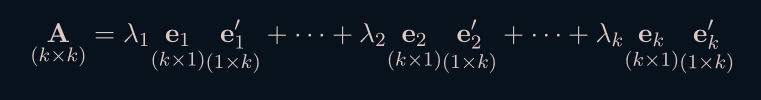
\includegraphics[width=0.5\linewidth]{desc.png}
        donte $ \lambda_1 , \lambda_2 , ... , \lambda_k  $ son los
        valores propios de $ A  $  y $ e_1 , ... , e_k   $ son los
        vectores propios normalizados asociados, entonces $ e_j'e_j = 1
        $para $ i = 1,2,3,4,...,k  $ y $ e_i e_j != 0   $ para $ i != j
        $
        \\
        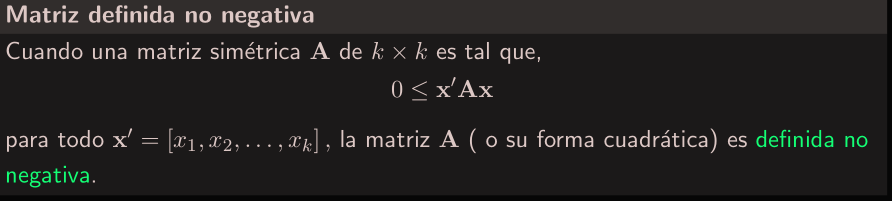
\includegraphics[width=0.5\linewidth]{pos.png}
        \\

         \color{red} mirar el ejemplo 2 en el notebook \color{white}


    \section{definicon matriz positiva}
        una matriz se define \color{red} no negativa \color{white} sii
        \color{red} sus valores propios son maores o iguales a 0
        \color{white}

        \\ una matriz es definida \color{blue} positiva \color{white}
        sii \color{red} todos sus valores propios son positivos
        \color{white}

        \begin{itemize}
            \item {si los elementos de un vector $ x = (x_1 , x_2 , ...
                , x_n )  $ son valores de p variables aleatorias $ X_1
            , X_2 , ...., X_N  $  estos elementos pueden considerarse
            como un punto en el espacio p dimensional y las distancias del
            punto al origen pueden interpretarse en terminos de la desviacion
            estándar }
            \item {se puede tener en cuenta la variabilidad de las observaciones}
            \item {los puntos con la misma \color{blue} incertidumbre
                \color{white} se consideran de igual distancia  al origen}
        \end{itemize}
        \begin{figure}[h!]
            \centering
            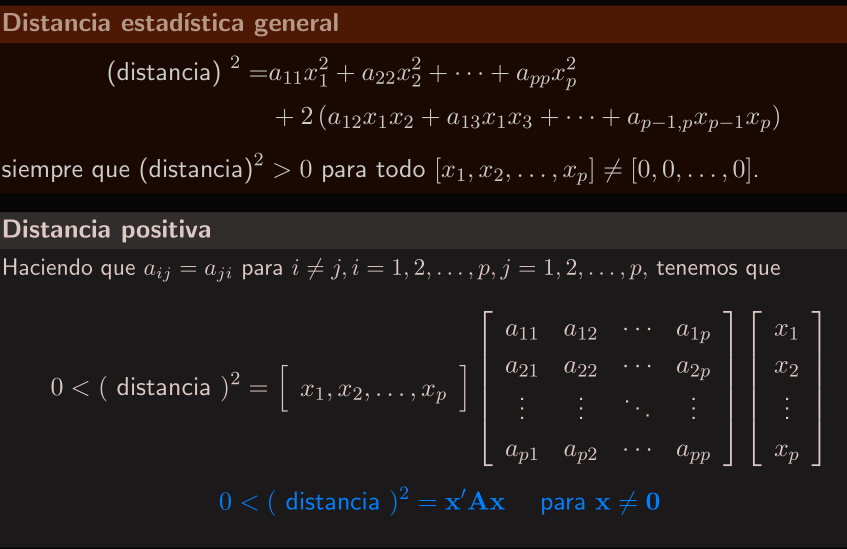
\includegraphics[width=0.5\linewidth]{dispos.png}
            \caption{Distancia Positiva}
            \label{fig:dispos}
        \end{figure}
            y ya

    \section{Dudas}

        \begin{itemize}
            \item {\color{yellow} que es $ e_x   $ en la formula de la
                descomposicion espectral? \color{white} }
        \end{itemize}




















    %=======================NOTES ENDS HERE===================%

    % bib stuff
    \nocite{*}
    \addtocontents{toc}{{}}
    \addcontentsline{toc}{section}{\refname}
    \bibliographystyle{plain}
    \bibliography{../Bibliography}
\end{document}
